\problemname{Patrick's Triangle}

%\illustration{0.5}{triangle.pdf}{The first six triangle numbers.
%Wikimedia Commons, CC BY-SA 3.0.}

Patrick is an unknown mathematician that wanted to become famous. Patrick had heard that the mathematician Blaise Pascal had became famous because of his triangle, Pascal's triangle.

\begin{center}
\begin{tabular}{rccccccccc}
&    &    &    &    &  1\\\noalign{\smallskip\smallskip}
&    &    &    &  1 &    &  1\\\noalign{\smallskip\smallskip}
&    &    &  1 &    &  2 &    &  1\\\noalign{\smallskip\smallskip}
&    &  1 &    &  3 &    &  3 &    &  1\\\noalign{\smallskip\smallskip}
&  1 &    &  4 &    &  6 &    &  4 &    &  1\\\noalign{\smallskip\smallskip}
\end{tabular}
\end{center}

Patrick thought that if he could come up with his own triangle, Patrick's triangle, then he maybe too would become famous. 
After thinking about it for a long while, he came up with the following construction:

\begin{enumerate}

\item{Along both the left side and right side of the triangle put the triangle numbers $1,3,6,10,15,21,\ldots$}


\begin{center}
\begin{tabular}{rccccccccc}
&    &    &    &    &  1\\\noalign{\smallskip\smallskip}
&    &    &    &  3 &    &  3\\\noalign{\smallskip\smallskip}
&    &    &  6 &    &   &    &  6\\\noalign{\smallskip\smallskip}
&    &  10 &    &   &    &   &    &  10\\\noalign{\smallskip\smallskip}
&  15 &    &   &    &   &    &   &    &  15\\\noalign{\smallskip\smallskip}
\end{tabular}
\end{center}

\item{Fill in the inside of the triangle by adding the number above and to the left with the number above and to the right, in the same way as Pascal's triangle is constructed.}

\begin{center}
\begin{tabular}{rccccccccc}
&     &     &    &    &  1\\\noalign{\smallskip\smallskip}
&     &     &    &  3 &    &  3\\\noalign{\smallskip\smallskip}
&     &     &  6 &    & 6  &    &  6\\\noalign{\smallskip\smallskip}
&     &  10 &    & 12  &    & 12  &    &  10\\\noalign{\smallskip\smallskip}
&  15 &     & 22  &    &  24  &    &  22  &    &  15\\\noalign{\smallskip\smallskip}
\end{tabular}
\end{center}

\end{enumerate}

Patrick knew that in order for his triangle to make him famous, he needed to make sure no one else had invented it before him. So he searched through the On-Line Encyclopedia of Integer Sequences (OEIS.org), and luckily his triangle was missing from OEIS. 

Now there was just one thing left to do, to upload his triangle to OEIS and become famous. To do this, Patrick calculated the first $10^6$ rows of the triangle by hand. But before he uploaded his triangle to OEIS, he wanted to make sure there were no errors in his calculations. Can you help him check his calculations?


\begin{minipage}{\textwidth}
\begin{center}

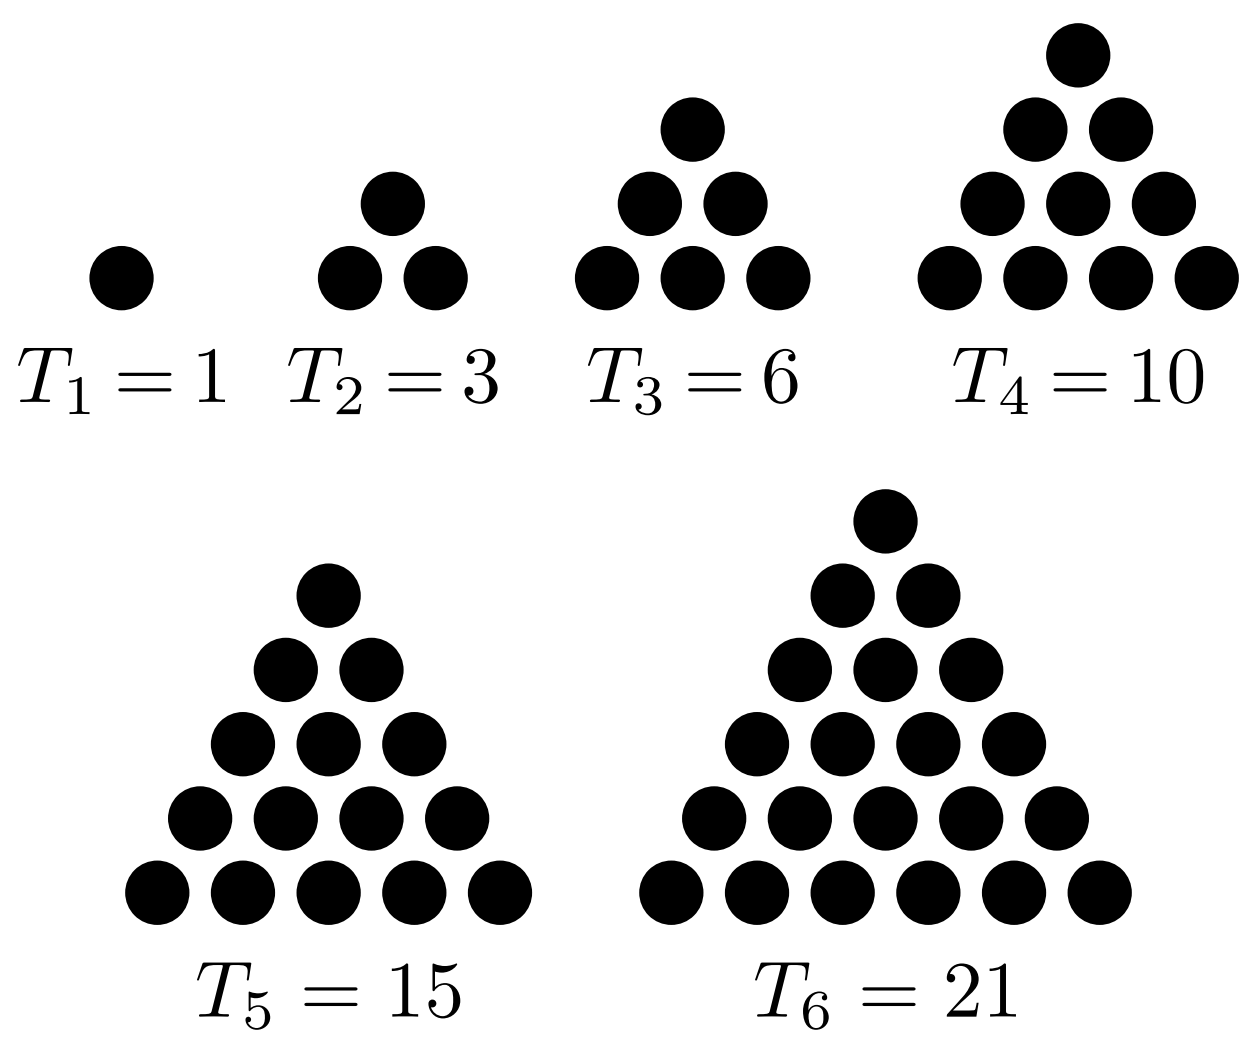
\includegraphics[width=.5\textwidth]{triangle.png}

The first 6 triangle numbers. Wikimedia Commons, CC BY-SA 3.0.
\end{center}
\end{minipage}


\section*{Input}
The first line consists of one integer $Q$ ($1 \leq Q \leq 2 \cdot 10^5$), the number of queries.
The next $Q$ lines consist of three space separated integers $N,K,X$ ($1 \leq K \leq N \leq 10^6$, $0 \leq X < 10^9+7$), 
where $X$ is the value Patrick got when he calculated the $K$-th number on the $N$-th row in Patrick's triangle mod $10^9 + 7$. 
Patrick wants to know if $X$ is correct or not.

\section*{Output}
For each of the $Q$ queries, output a single line with the string \texttt{Correct} if the $K$-th number on the $N$-th row in Patrick's triangle is equal to $X$ mod $10^9 + 7$, otherwise output the string \texttt{Incorrect}.
